% Figura 5: posiciones X/Y locales reproducidas de la hoja «Base por sector».
% Los puntos NO se presentan como coordenadas UTM ni sobre un mapa georreferenciado.
\begingroup
\setlength{\parskip}{0pt}
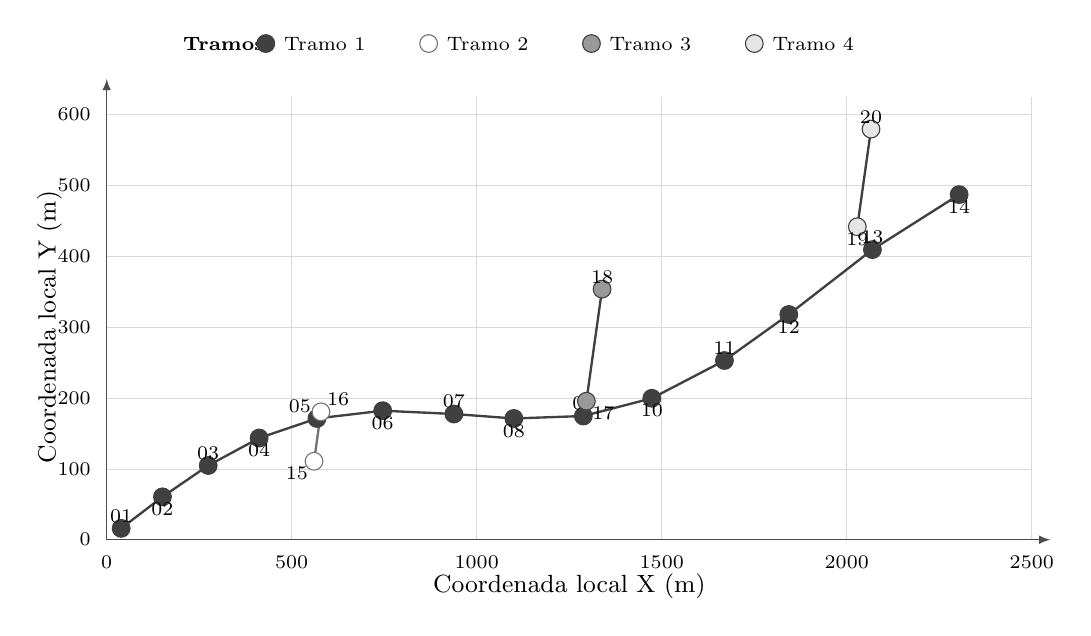
\begin{tikzpicture}[x=0.0047cm,y=0.0090cm,
  tramoUno/.style={draw=black!75,fill=black!75},
  tramoDos/.style={draw=black!55,fill=white},
  tramoTres/.style={draw=black!75,fill=black!40},
  tramoCuatro/.style={draw=black!75,fill=black!10}]
% Rejilla y ejes. Coordenadas originales en metros, escaladas únicamente para visualizar.
\foreach \xx in {0,500,1000,1500,2000,2500}{%
  \draw[black!15,line width=0.25pt] (\xx,0) -- (\xx,625);
  \node[below,font=\scriptsize] at (\xx,-9) {\xx};
}
\foreach \yy in {0,100,200,300,400,500,600}{%
  \draw[black!15,line width=0.25pt] (0,\yy) -- (2500,\yy);
  \node[left,font=\scriptsize] at (-17,\yy) {\yy};
}
\draw[black!70,-latex] (0,0)--(2550,0);
\draw[black!70,-latex] (0,0)--(0,650);
\node[font=\small] at (1250,-66) {Coordenada local X (m)};
\node[rotate=90,font=\small] at (-155,300) {Coordenada local Y (m)};
% Recorridos que enlazan solamente unidades consecutivas del mismo tramo.
\draw[line width=0.85pt,tramoUno,fill=none] (39.06,16.03) -- (150.66,60.54) -- (274.35,104.72) -- (411.99,143.49) -- (568.23,171.13) -- (745.86,182.04) -- (938.37,177.40) -- (1100.19,171.09) -- (1288.05,174.54) -- (1473.12,199.55) -- (1669.35,252.85) -- (1843.26,317.79) -- (2069.25,409.28) -- (2303.61,486.90);
\draw[line width=0.85pt,tramoDos,fill=none] (560.25,110.69) -- (579.00,180.44);
\draw[line width=0.85pt,tramoTres,fill=none] (1296.25,195.45) -- (1338.75,353.55);
\draw[line width=0.85pt,tramoCuatro,fill=none] (2028.50,441.62) -- (2065.50,579.26);
% Marcadores independientes por unidad, con etiquetas numeradas 01--20.
\filldraw[tramoUno,line width=0.4pt] (39.06,16.03) circle[x radius=3.2pt,y radius=3.2pt];
\node[font=\scriptsize,above,inner sep=2pt] at (39.06,16.03) {01};
\filldraw[tramoUno,line width=0.4pt] (150.66,60.54) circle[x radius=3.2pt,y radius=3.2pt];
\node[font=\scriptsize,below,inner sep=2pt] at (150.66,60.54) {02};
\filldraw[tramoUno,line width=0.4pt] (274.35,104.72) circle[x radius=3.2pt,y radius=3.2pt];
\node[font=\scriptsize,above,inner sep=2pt] at (274.35,104.72) {03};
\filldraw[tramoUno,line width=0.4pt] (411.99,143.49) circle[x radius=3.2pt,y radius=3.2pt];
\node[font=\scriptsize,below,inner sep=2pt] at (411.99,143.49) {04};
\filldraw[tramoUno,line width=0.4pt] (568.23,171.13) circle[x radius=3.2pt,y radius=3.2pt];
\node[font=\scriptsize,above left,inner sep=2pt] at (568.23,171.13) {05};
\filldraw[tramoUno,line width=0.4pt] (745.86,182.04) circle[x radius=3.2pt,y radius=3.2pt];
\node[font=\scriptsize,below,inner sep=2pt] at (745.86,182.04) {06};
\filldraw[tramoUno,line width=0.4pt] (938.37,177.40) circle[x radius=3.2pt,y radius=3.2pt];
\node[font=\scriptsize,above,inner sep=2pt] at (938.37,177.40) {07};
\filldraw[tramoUno,line width=0.4pt] (1100.19,171.09) circle[x radius=3.2pt,y radius=3.2pt];
\node[font=\scriptsize,below,inner sep=2pt] at (1100.19,171.09) {08};
\filldraw[tramoUno,line width=0.4pt] (1288.05,174.54) circle[x radius=3.2pt,y radius=3.2pt];
\node[font=\scriptsize,above,inner sep=2pt] at (1288.05,174.54) {09};
\filldraw[tramoUno,line width=0.4pt] (1473.12,199.55) circle[x radius=3.2pt,y radius=3.2pt];
\node[font=\scriptsize,below,inner sep=2pt] at (1473.12,199.55) {10};
\filldraw[tramoUno,line width=0.4pt] (1669.35,252.85) circle[x radius=3.2pt,y radius=3.2pt];
\node[font=\scriptsize,above,inner sep=2pt] at (1669.35,252.85) {11};
\filldraw[tramoUno,line width=0.4pt] (1843.26,317.79) circle[x radius=3.2pt,y radius=3.2pt];
\node[font=\scriptsize,below,inner sep=2pt] at (1843.26,317.79) {12};
\filldraw[tramoUno,line width=0.4pt] (2069.25,409.28) circle[x radius=3.2pt,y radius=3.2pt];
\node[font=\scriptsize,above,inner sep=2pt] at (2069.25,409.28) {13};
\filldraw[tramoUno,line width=0.4pt] (2303.61,486.90) circle[x radius=3.2pt,y radius=3.2pt];
\node[font=\scriptsize,below,inner sep=2pt] at (2303.61,486.90) {14};
\filldraw[tramoDos,line width=0.4pt] (560.25,110.69) circle[x radius=3.2pt,y radius=3.2pt];
\node[font=\scriptsize,below left,inner sep=2pt] at (560.25,110.69) {15};
\filldraw[tramoDos,line width=0.4pt] (579.00,180.44) circle[x radius=3.2pt,y radius=3.2pt];
\node[font=\scriptsize,above right,inner sep=2pt] at (579.00,180.44) {16};
\filldraw[tramoTres,line width=0.4pt] (1296.25,195.45) circle[x radius=3.2pt,y radius=3.2pt];
\node[font=\scriptsize,below right,inner sep=2pt] at (1296.25,195.45) {17};
\filldraw[tramoTres,line width=0.4pt] (1338.75,353.55) circle[x radius=3.2pt,y radius=3.2pt];
\node[font=\scriptsize,above,inner sep=2pt] at (1338.75,353.55) {18};
\filldraw[tramoCuatro,line width=0.4pt] (2028.50,441.62) circle[x radius=3.2pt,y radius=3.2pt];
\node[font=\scriptsize,below,inner sep=2pt] at (2028.50,441.62) {19};
\filldraw[tramoCuatro,line width=0.4pt] (2065.50,579.26) circle[x radius=3.2pt,y radius=3.2pt];
\node[font=\scriptsize,above,inner sep=2pt] at (2065.50,579.26) {20};
% Leyenda: tipo de símbolo, no magnitudes de ubicación.
\begin{scope}[shift={(180,700)}]
 \node[anchor=west,font=\scriptsize] at (0,0) {\textbf{Tramos:}};
 \foreach \style/\name/\dx in {tramoUno/1/250,tramoDos/2/690,tramoTres/3/1130,tramoCuatro/4/1570}{%
   \filldraw[\style] (\dx,0) circle[x radius=3.2pt,y radius=3.2pt];
   \node[anchor=west,font=\scriptsize] at (\dx+23,0) {Tramo \name};
 }
\end{scope}
\end{tikzpicture}
\endgroup
